
\item O carrinho de montanha-russa tendo massa $m$, é solto do repouso no ponto $A$. Se a pista precisa ser projetada de maneira que o carrinho não a deixe em $B$, determine a altura necessária $h$. Além disso, determine a velocidade do carrinho quando ele chega ao ponto $C$. Despreze o atrito.

\import{answers/}{answer-12}

\begin{flushleft}
    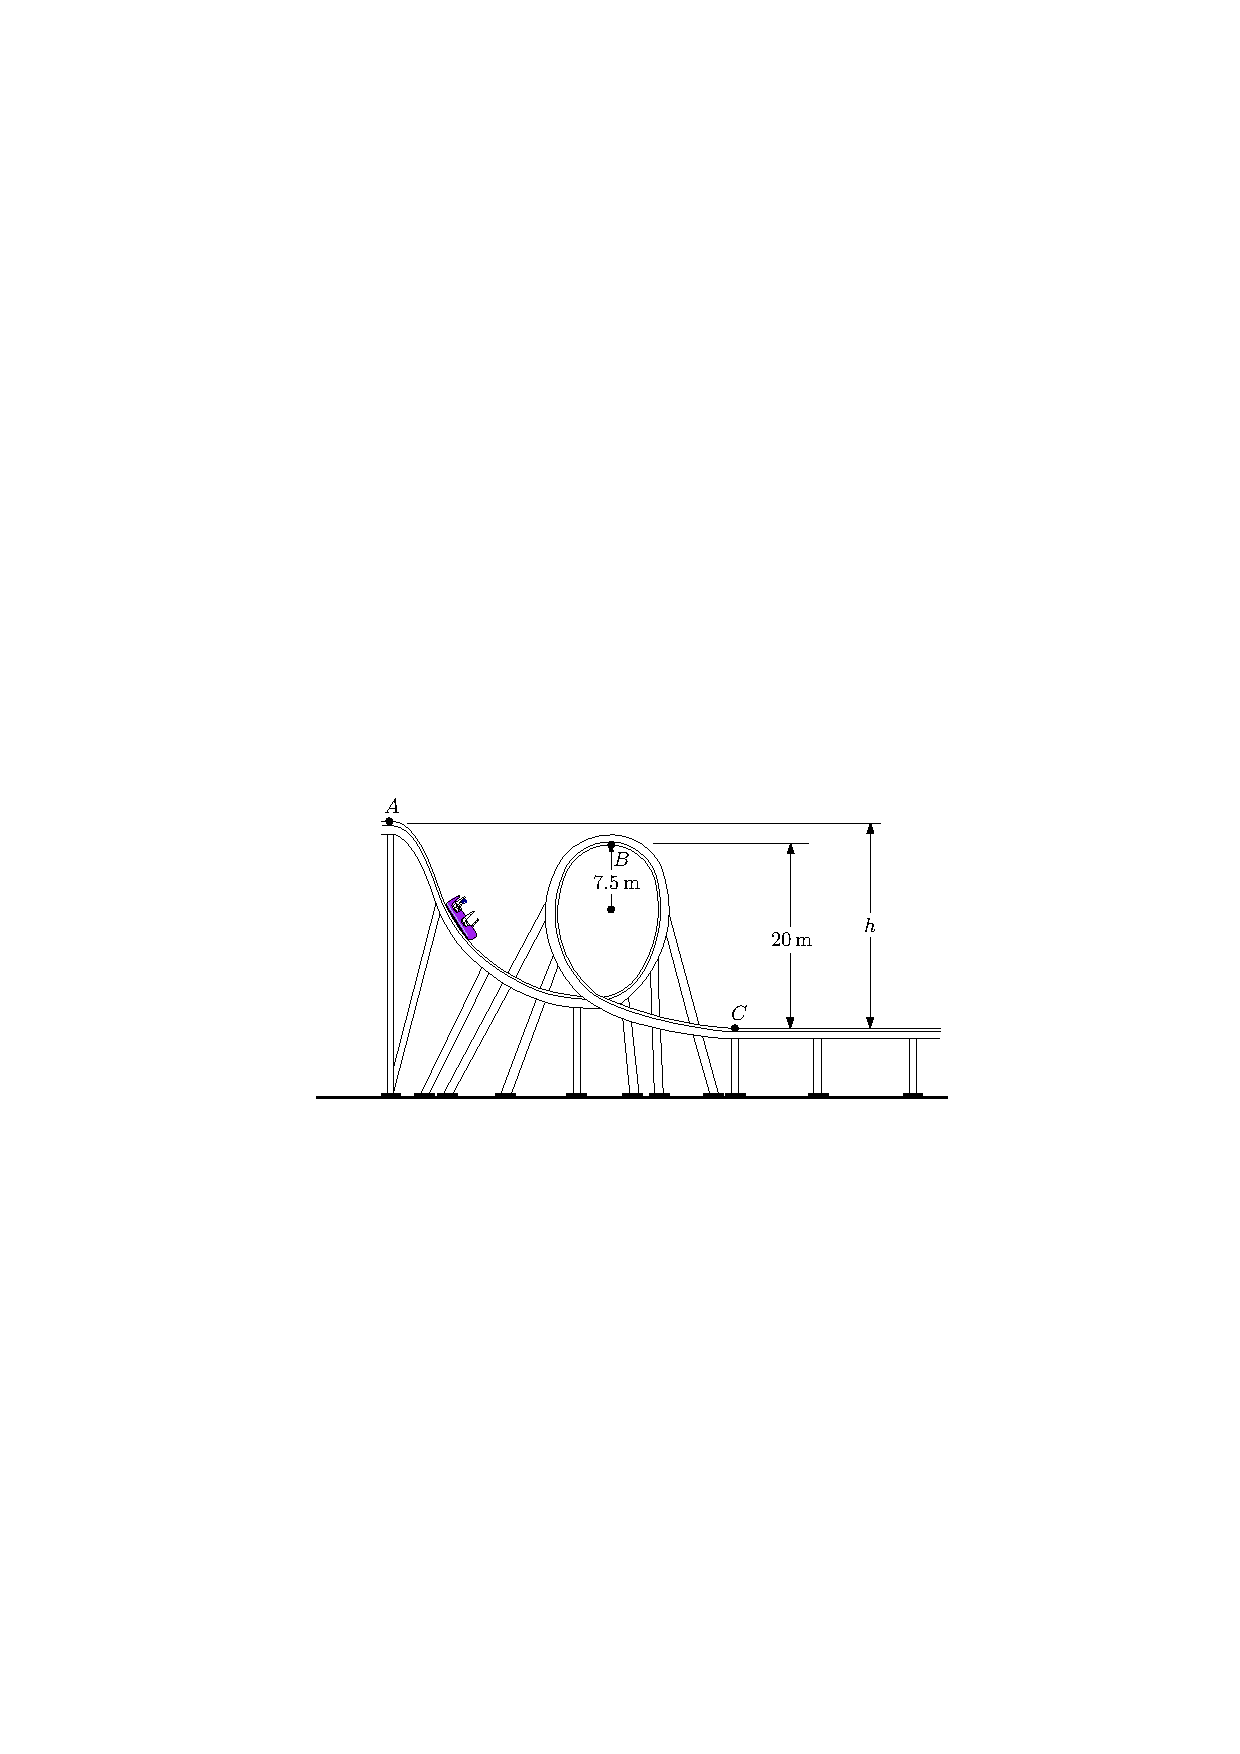
\includegraphics[scale=1.3]{images/draw_12.pdf}
\end{flushleft}